\documentclass[12pt, openany]{report}
\usepackage[utf8]{inputenc}
\usepackage[T1]{fontenc}
\usepackage[a4paper,left=2cm,right=2cm,top=2cm,bottom=2cm]{geometry}
\usepackage[frenchb]{babel}
\usepackage[pdftex]{graphicx}
\usepackage{amsmath,amsfonts,amssymb}
\usepackage{hyperref}
\usepackage{color}
\usepackage[table]{xcolor}
\usepackage{listings}
\usepackage{enumitem}
\usepackage{pifont}
\usepackage{ragged2e}
\usepackage{tabto}


\setlength{\parindent}{0cm}
\setlength{\parskip}{1ex plus 0.5ex minus 0.2ex}
\newcommand{\hsp}{\hspace{20pt}}
\newcommand{\HRule}{\rule{\linewidth}{0.5mm}}
%\renewcommand{\thesection}{\Roman{section}}
\renewcommand{\thesection}{\arabic{section}} 


%contenu du document
\begin{document}


\begin{titlepage}
  \begin{sffamily}
  \begin{center}
	
\includegraphics[scale=0.5]{ub.png}~\\[1cm]

    \textsc{\Large MASTER 2 Informatique RCI }\\[1.5cm]
    2021-2022

    % Titre
    \rule{1\linewidth}{2pt}
     \\[1cm]
    { \huge \bfseries Rapport de PFE :\\
    Déploiement d'un VPN sur des équipements mobiles ou IoT\\[1cm] }
    \rule{1\linewidth}{2pt}
    \\[1cm]
    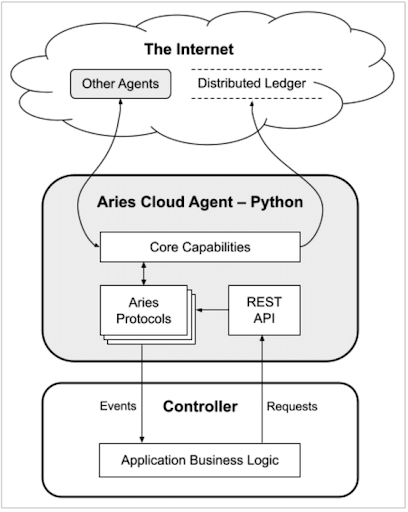
\includegraphics[scale=0.55]{couv.png}
    \\ %[1cm]

    % Membres du groupe
   \vfill
      \begin{center}
        %\hspace*{3.1cm}
        \Large	 Alexis Henquinet \hspace*{1cm} Mohamed Diallo \hspace*{1cm} Sara Real Santos
      \end{center}
 
    % Bas de la page
 
  \end{center}
  \end{sffamily}
\end{titlepage}

\newpage

\renewcommand{\contentsname}{Sommaire}
%\addcontentsline{toc}{section}{Remerciements}
\tableofcontents
\newpage

\section{Introduction}
\noindent 
\begin{flushleft}
TODO
\end{flushleft}

\section{Étude de l'existant}
\noindent 
\begin{flushleft}
TODO
\end{flushleft}

\section{Besoins}
\noindent 
\begin{flushleft}
TODO
\end{flushleft}
\subsection{Besoins fonctionnels}
\noindent 
\begin{flushleft}
TODO
\end{flushleft}
\subsection{Besoins utilisateurs non fonctionnels}
\noindent 
\begin{flushleft}
TODO
\end{flushleft}

\section{Scénarios fonctionnels}
\noindent 
\begin{flushleft}
TODO
\end{flushleft}

\section{Architecture et implémentation}
\noindent 
\begin{flushleft}
TODO
\end{flushleft}

\section{Analyse du fonctionnement \& Tests}
\noindent 
\begin{flushleft}
TODO
\end{flushleft}

\section{Conclusion}
\noindent 
\begin{flushleft}
TODO
\end{flushleft}
\subsection{Limitations}
\noindent 
\begin{flushleft}
TODO
\end{flushleft}
\subsection{Extensions}
\noindent 
\begin{flushleft}
TODO
\end{flushleft}

\section{Bibliographie}
\noindent 
\begin{flushleft}
TODO
\end{flushleft}

\section{Annexe}
\noindent 
\begin{flushleft}
TODO
\end{flushleft}
\end{document}

